The results in section \ref{res:amazon} show that there is a linear correlation between the scale, number of nodes and performance. Using this information a model can be made.

\begin{figure}[!h]
	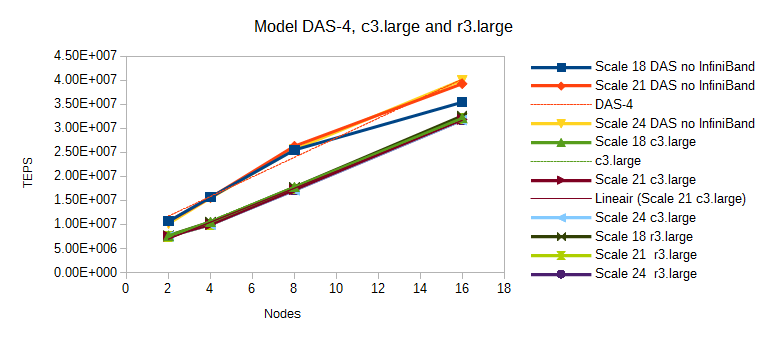
\includegraphics[width=\textwidth]{images/model_figure_1.png}
	\caption{The linear behavior for the DAS-4,c3.large and r3.large.}
	\label{fig:model_first}
\end{figure}

Two examples of these equations can be made from figure \ref{fig:model_first}.
First the equation for the DAS-4:
%\begin{equation}
%f(x) = 2034724.34782609 * X + 7702517.39130435
%\end{equation}

\begin{equation}
TEPS(x) = 2.03 * X + 7.70
\end{equation}

Second the equation for Amazon EC2:
\begin{equation}
f(x) = 1.76 * X + 3.45
\end{equation}
Where X is the number of nodes used for the application. Both equations return a value in $10^6$ TEPS (MTEPS).

As can be seen from these two equations the slope and the starting value depend on the architecture on which it runs. To discover these values empirically a few experiments need to be done with the hardware of choice. When these numbers have been found they can be inserted in the formula and.

The model made can only predict the performance of the as a function of the number of nodes for large scale. To calculate the point where maximum parallelism can be achieved and the point of the diminishing return cannot be calculated.